
\renewcommand{\theequation}{\theenumi}
\begin{enumerate}[label=\thesection.\arabic*.,ref=\thesection.\theenumi]
\numberwithin{equation}{enumi}
	
\item Show that $\vec{E},\vec{F},\vec{G},\vec{H}$ lies on a circle.
\\
\solution Let $\vec{V}$ be a general vector that satisfies the circle equation.
\\
Then, $\norm{V-O}=r$ will be the equation,
\\
where $\vec{O},R$ are Centre of circle, and radius respectively.
\\
Find a point $\vec{O}$ that is equidistant from the vertices of $\triangle EFG$ for $e = 1.010, f = 1.212, g = 0.940$.
\begin{align}
\label{eq:ec}
\norm{E-O}=
\norm{F-C}=
\norm{G-C}=R
\end{align}
%By equating .\eqref{eq:ec}=.\eqref{eq:fc} and equating .\eqref{eq:fc}=.\eqref{eq:gc}, we can find the value of $\vec{C}$.
%\begin{align}
%\norm{\myvec{5.313-x\\2.657-y}}=\norm{\myvec{4.471-x\\2.236-y}}
%\\
%\norm{\myvec{4.471-x\\2.236-y}}=\norm{\myvec{5.119-x\\1.460-y}}
%\end{align}
%By solving the above two equations we get the value of $\vec{C}$
%\\
%$\therefore \vec{C}=\myvec{5.075\\2.081}$
%\\
%and by substituting the value of $\vec{C}$ in the equation .\eqref{eq:ec}, we get the value of r.
%$\therefore r=0.622$.
%\\
%To prove that Quadrilateral EFGH is a cyclic, then H should aslo lie on the circle.
%\\ 
%$\vec{H}$ should satisfy the general circle equation, $\norm{V-C}=r$.
%\\
%$\norm{H-C}=r$
%\begin{align}
%\norm{\myvec{5.545-5.075\\2.489-2.081}}=
%\norm{\myvec{0.470\\0.408}}=0.622
%\end{align}
%As $\vec{H}$ satisfies the general circle equation.
%\newline
%$\therefore$ Quadrilateral EFGH is a cyclic quadrilateral.
From \eqref{eq:ec},
\begin{align}
\label{eq:circle_const_EF}
\norm{\vec{E}-\vec{O}}^2 - \norm{\vec{F}-\vec{O}}^2  = 0
\end{align}
\begin{multline}
\implies \brak{\vec{E}-\vec{O}}^T\brak{\vec{E}-\vec{O}} 
\\
- \brak{\vec{F}-\vec{O}}^T\brak{\vec{F}-\vec{O}} = 0
\end{multline}
%
which can be simplified as
\begin{align}
\label{eq:circle_const_chord_ef}
\brak{\vec{E}-\vec{F}}^T\vec{O} =   \frac{\norm{\vec{E}}^2- \norm{\vec{F}}^2}{2}
\end{align}
Similarly,
\begin{align}
\label{eq:circle_const_chord_fg}
\brak{\vec{F}-\vec{G}}^T\vec{O} =  \frac{\norm{\vec{F}}^2- \norm{\vec{G}}^2}{2}
\end{align}
%
\eqref{eq:circle_const_chord_ef} and \eqref{eq:circle_const_chord_fg}, can be combined to form the matrix equation 
%
\begin{align}
\vec{N}^T\vec{O} &= \vec{g}
\\
\implies \vec{O} &= \vec{N}^{-T} \vec{g}
\label{eq:circle_const_chord_mat}
\end{align}
%
where 
%
\begin{align}
%\label{eq:circle_const_chord_mat}
\vec{N} &= \myvec{\vec{E}-\vec{F} & \vec{F}-\vec{G}}
\\
\vec{g} &= \frac{1}{2}\myvec{\norm{\vec{E}}^2- \norm{\vec{F}}^2 \\ \norm{\vec{F}}^2- \norm{\vec{G}}^2}
\end{align}
%
$\vec{O}$ can be computed using 
%
the python code below
%
\begin{lstlisting}
codes/quad.py
\end{lstlisting}
%
and the equivalent latex-tikz code to draw Fig. \ref{fig:tri_ccentre} is
%
\begin{lstlisting}
figs/quad.tex
\end{lstlisting}
%
\begin{figure}[!ht]
	\begin{center}
		\resizebox{\columnwidth}{!}{%Code by GVV Sharma
%December 9, 2019
%released under GNU GPL
%Locating the circumcentre

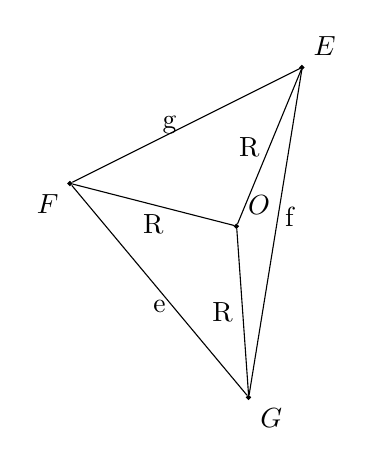
\begin{tikzpicture}
[scale=3.5,>=stealth,point/.style={draw,circle,fill = black,inner sep=0.5pt},]

%Triangle sides
\def\e{1.010}
\def\f{1.212}
\def\g{0.940}
 
%Coordinates of A
%\def\p{{\a^2+\c^2-\b^2}/{(2*\a)}}
%\def\p{0.5}
%\def\q{{sqrt(\c^2-\p^2)}}

%Labeling points
\node (E) at (5.313,2.657)[point,label=above right:$E$] {};
\node (F) at (4.471,2.236)[point,label=below left:$F$] {};
\node (G) at (5.119,1.460)[point,label=below right:$G$] {};

%Circumcentre

\node (O) at (5.075,2.081)[point,label=above right:$O$] {};

%Drawing triangle EFG
\draw (E) -- node[left] {$\textrm{g}$} (F) -- node[below] {$\textrm{e}$} (G) -- node[right,yshift=2mm] {$\textrm{f}$} (E);
%Drawing OA, OB, OC
\draw (O) -- node[left] {$\textrm{R}$} (E);
\draw (O) -- node[below] {$\textrm{R}$} (F);
\draw (O) -- node[left] {$\textrm{R}$} (G);

%\tkzMarkAngle[fill=blue!50,size=.3](C,B,O)
%\tkzMarkAngle[fill=blue!50,size=.3](O,C,B)


%\tkzMarkAngle[fill=red!50](O,A,C)
%\tkzMarkAngle[fill=red!50](A,C,O)


%\tkzMarkAngle[fill=orange!50,size=.3](B,A,O)
%\tkzMarkAngle[fill=orange!50,size=.3](O,B,A)

%\tkzLabelAngle[pos=0.5](O,C,B){$\theta_1$}
%\tkzLabelAngle[pos=0.5](O,B,C){$\theta_1$}
%\tkzLabelAngle[pos=0.5](O,A,B){$\theta_2$}
%\tkzLabelAngle[pos=0.5](O,B,A){$\theta_2$}
%\tkzLabelAngle[pos=1.5](O,A,C){$\theta_3$}
%\tkzLabelAngle[pos=1.5](O,C,A){$\theta_3$}

\end{tikzpicture}
}
	\end{center}
	\caption{Circumcentre $O$ of $\triangle EFG$}
	\label{fig:tri_ccentre}	
\end{figure}
%
\item $\therefore \vec{O}=\myvec{5.075\\2.081}$
\item In $\triangle OFG$, $OF=OG = R$.  Such a triangle is known as an {\em isoceles triangle}.
%
\item Show that $\angle OFG = \angle OGF$.  In an isoceles triangle, opposite sides and corresponding opposite angles are equal.
\label{prob:tri_ang_side_eq}
\\
\solution Using the sine formula ,%
\begin{align}
\frac{\sin \angle OFG}{R} &= \frac{\sin \angle OGF}{R}
\\
\implies \sin \angle OFG &= \sin \angle OGF
\end{align}
%
\item  Show that $\angle FOG = 2\angle E$.
\label{prob:tri_ccentre_subtend}
%
\\
\solution In Fig. \ref{fig:tri_ccentre}, 
%
\begin{align}
%
\label{eq:tri_ccentre_A23}
E &= \theta_2+\theta_3
\\
F &= \theta_1+\theta_2
\\
G &= \theta_3+\theta_1
\\
\implies 2\brak{\theta_1+\theta_2+\theta_3} &= E+G+H =180\degree
\\
\implies \theta_1+\theta_2+\theta_3 &= 90\degree
\label{eq:tri_ccentre_sum_123}
\end{align}
%
From \eqref{eq:tri_ccentre_A23} and \eqref{eq:tri_ccentre_sum_123},
%
\begin{align}
%
\label{eq:tri_ccentre_A1}
E &= 90\degree - \theta_1
\end{align}
%
Also, in $\triangle OFG$, all angles add up to $180\degree$.  Hence, 
%
\begin{align}
\angle FOG + 2\theta_1 &= 180\degree
\\
\implies \angle FOG &= 180\degree - 2\theta_1 = 2 \brak{90\degree - \theta_1}
%\\
%&
= 2\angle E
\end{align}
%
upon substituting from \eqref{eq:tri_ccentre_A1}.
%
\item Let $\vec{L}$ be the mid point of $FG$.  Show that $OL \perp FG$.
\label{prob:tri_perp_bisect}
%
\\
\solution From \eqref{eq:circle_const_chord_ef}, 
%
\begin{align}
\brak{\vec{F}-\vec{G}}^T\vec{O} &=   \frac{\norm{\vec{F}}^2- \norm{\vec{G}}^2}{2}
\\
\implies \brak{\vec{F}-\vec{G}}^T\vec{O} &=   \frac{1}{2}\brak{\vec{F}- \vec{G}}^T\brak{\vec{F}+ \vec{G}}
\\
\implies \brak{\vec{F}-\vec{G}}^T&\brak{\vec{O} - \frac{\vec{F}+\vec{G}}{2}} = 0
\\
\text{or, } \brak{\vec{F}-\vec{G}}^T&\brak{\vec{O} - \vec{L}} = 0
\end{align}
%
$\because \vec{L} = \frac{\vec{F}+\vec{G}}{2}$ is the mid point of $FG$.  From \eqref{eq:tri_baudh_orth} we then conclude that $OL \perp FG$.
%
\item Perpendicular bisectors of a triangle meet at the circumcentre.
%
\item In the isosceles $\triangle OFG$, if $FL = LG$, $OL \perp FG$.
\label{them:isos_pb}

\item Show that 
\begin{align}
\label{eq:tri_crad_R}
\frac{e}{\sin E} = \frac{f}{\sin F} = \frac{g}{\sin G} = 2R.
\end{align}
%
\solution In $\triangle OFG$, using the cosine formula, 
\begin{align}
\cos 2A = \frac{R^2+R^2 - e^2}{2R^2} = 1 -\frac{e^2}{2R^2}
\label{eq:crad_cos2a}
\end{align}
%
Using the sine formula, 
\begin{align}
\frac{\sin 2E}{e} &= \frac{\sin \theta_1}{R} = \frac{\sin\brak{90\degree- E}}{R}
\\
\implies \sin 2E &= \frac{a\cos E}{R}
\label{eq:crad_sin2a}
\end{align}
%
from \eqref{eq:tri_ccentre_A1} and Baudhanya theorem. 
\begin{align}
\cos^2 2E + \sin^2 2E&= 1
\\
\implies \brak{1 -\frac{e^2}{2R^2}}^2 + \brak{\frac{e\cos E}{R}}^2 &= 1
\end{align}
%
upon substituting from \eqref{eq:crad_cos2a}  and \eqref{eq:crad_sin2a}.  Letting
%
\begin{align}
\label{eq:tri_crad_x}
x = \brak{\frac{e}{R}}^2,
\end{align}
%
in the previous equation yields
%
\begin{align}
 \brak{1 -\frac{x}{2}}^2 + x\cos^2 E&= 1
\\
\implies 1 - \frac{x^2}{4} -x + x\cos^2 E&= 1
\\
\implies x\brak{1-\cos^2 E} - \frac{x^2}{4} &= 0
\\
x\sin^2 E - \frac{x^2}{4} &= 0
\\
\implies x\brak{\sin^2 E - \frac{x}{4}} &= 0
\\
\text{or, } \frac{x}{4} - \sin^2 E &=0
\end{align}
%
$\because x \ne 0$.  Thus, substituting from \eqref{eq:tri_crad_x},
\begin{align}
x = \brak{\frac{e}{R}}^2 &= 4 \sin^2 E 
\\
\implies \frac{e}{R} &= 2\sin E,
\\
\text{or, }\quad \frac{e}{\sin E} = 2R
%\label{eq:circ_chord_len}
\end{align}
%
\item Show that 
\label{eq:cos2x}
\begin{align}
\cos 2E &= 1 -2\sin^2 E = 2\cos^2 E - 1 
\\
&= \cos^2 E - \sin^2E \quad \text{ and }
\\
\sin 2E &= 2 \sin E \cos E
\label{eq:sin2x}
\end{align}
\item Find $R$.
\\
\solution
\begin{align}
ar\brak{\triangle EFG} = \frac{1}{2}fg \sin E = \frac{efg}{4R}&
\\
\implies R = \frac{efg}{4s\sqrt{\brak{s-e}\brak{s-f}\brak{s-g}}}&
\end{align}
%
upon substituting from \eqref{eq:tri_crad_R} and using Hero's formula.
%
\item Show that
%
\begin{align}
\label{eq:circ_area_chord}
ar\brak{\triangle OFG} = \frac{1}{2}R^2\sin 2E
\end{align}
%
\item Find the circumradius of $\triangle EFG$ for $e =1.010, f =1.212, g =0.940$.
%
\\
\solution The following python code calculates the circumradius
\begin{lstlisting}
codes/quad.py
\end{lstlisting}
$\therefore \vec{R}=0.622$

\item To prove QuadrilateralEFGH to be cyclic
$\vec{H}$ should satisfy the general circle equation, $\norm{V-C}=R$.
\\
$\norm{H-C}=R$
\begin{align}
\norm{\myvec{5.545-5.075\\2.489-2.081}}=
\norm{\myvec{0.470\\0.408}}=0.622
\end{align}
As $\vec{H}$ satisfies the general circle equation.
\newline
$\therefore$ Quadrilateral EFGH is a cyclic quadrilateral.
\end{enumerate}
